% \section{Comparison Human and GPT4 and GPT4-V}

% \begin{figure}[h!t]
% \centering
% 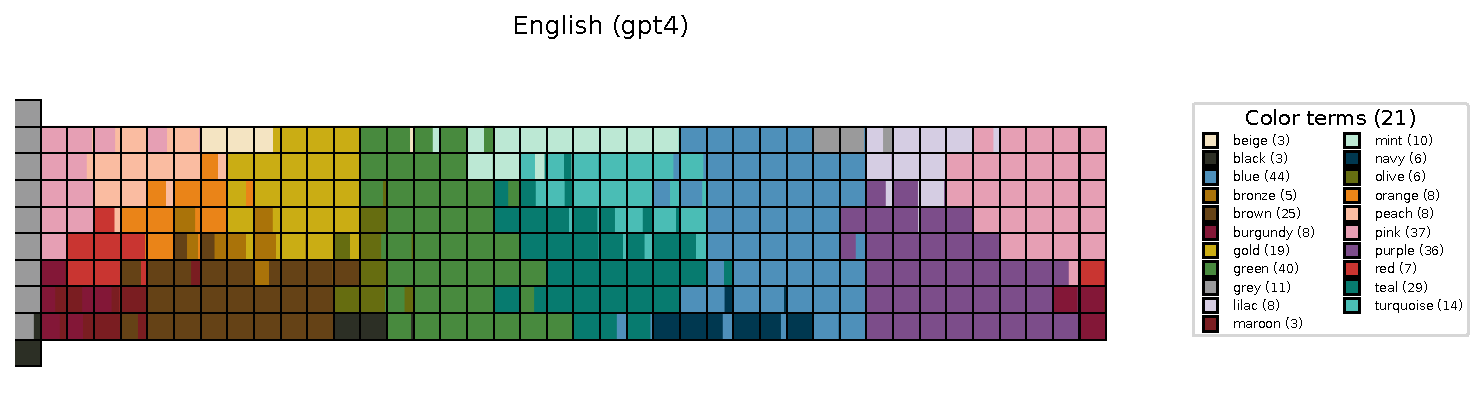
\includegraphics[width=\linewidth]{images/mode_maps_gpt4/English (gpt4).pdf}
% \hfill
% 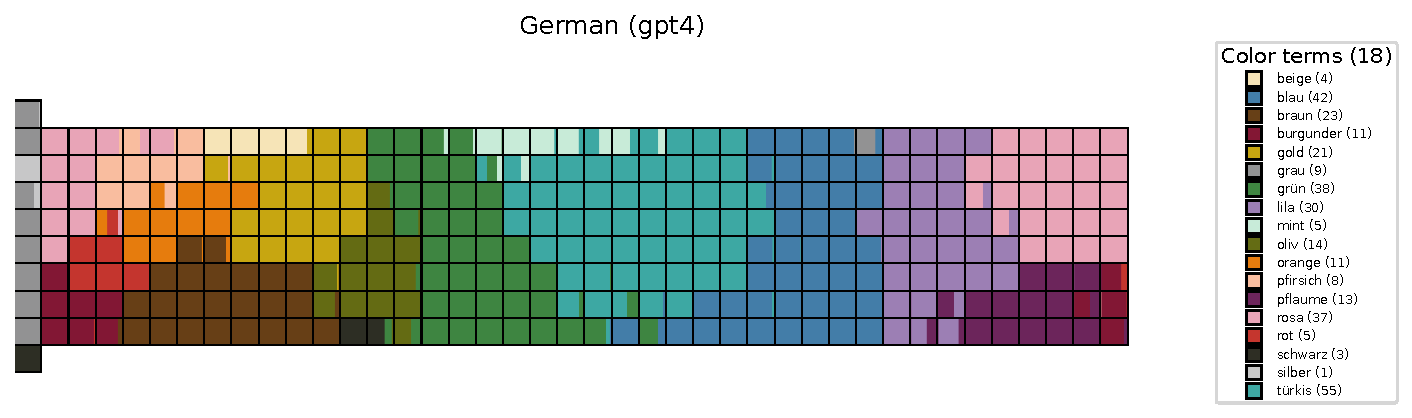
\includegraphics[width=\linewidth]{images/mode_maps_gpt4/German (gpt4).pdf}
% 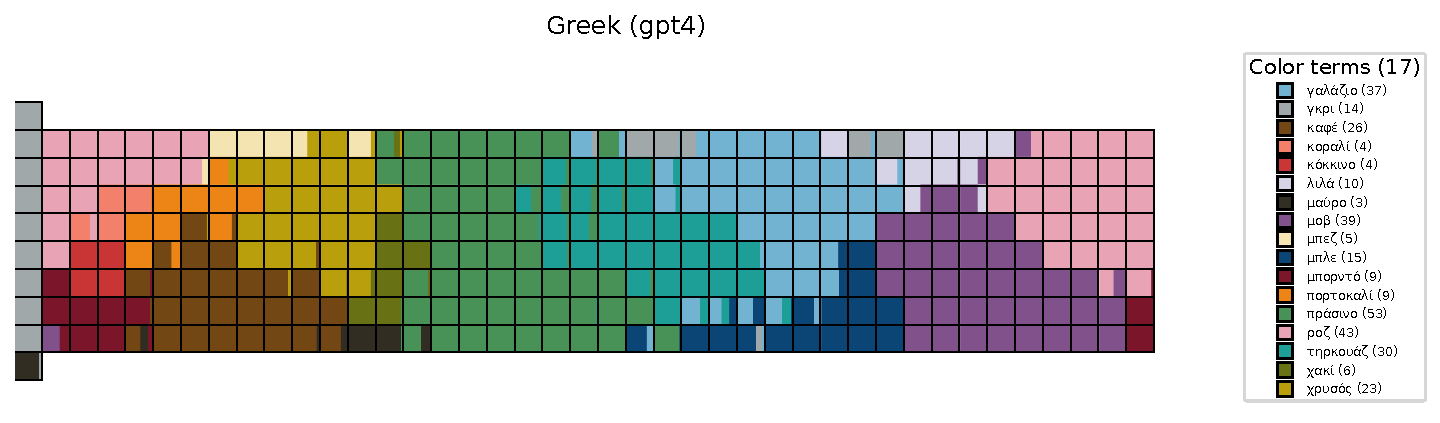
\includegraphics[width=\linewidth]{images/mode_maps_gpt4/Greek (gpt4).pdf}
% 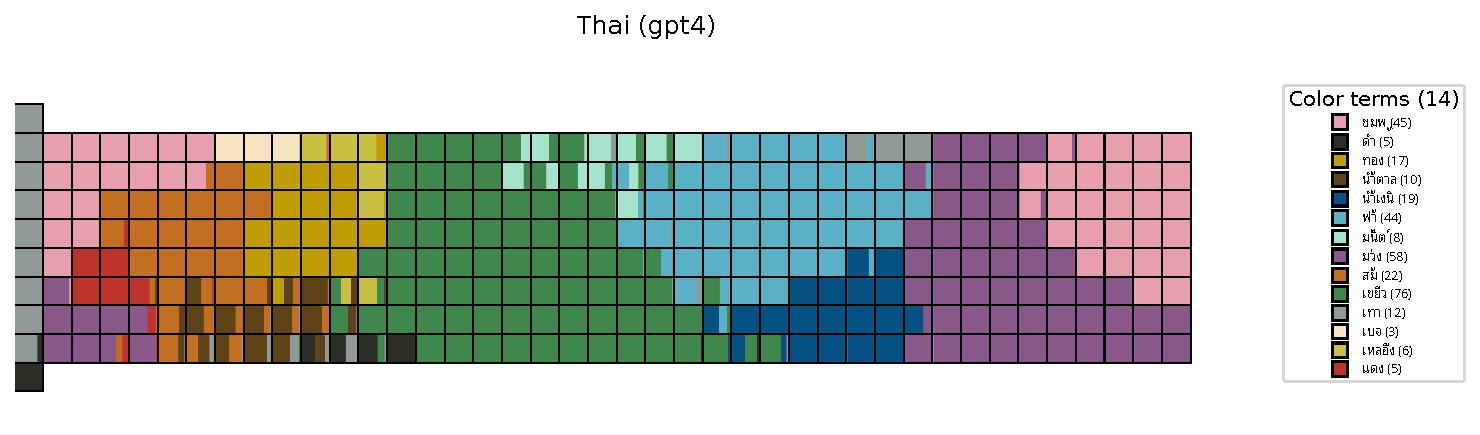
\includegraphics[width=\linewidth]{images/mode_maps_gpt4/Thai (gpt4).pdf}
% 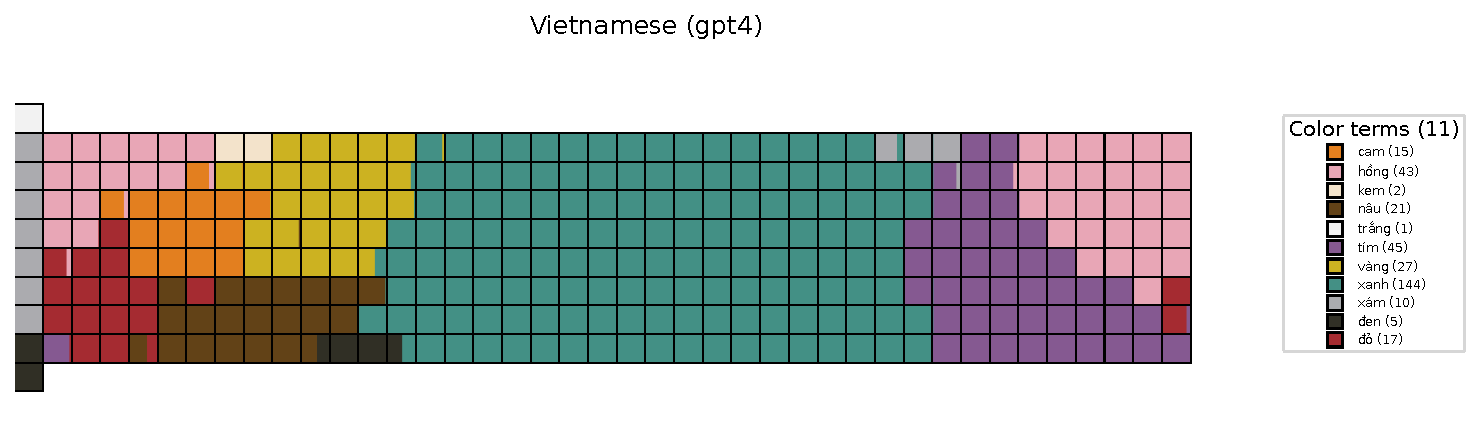
\includegraphics[width=\linewidth]{images/mode_maps_gpt4/Vietnamese (gpt4).pdf}
% \caption[GPT Proportion Plots]{Proportion plots for English, German, Greek, Thai, Vietnamese elicited from GPT4}
% \label{fig:mode-maps-gpt}
% \end{figure}

% \begin{figure}[h!t]
% \centering
% 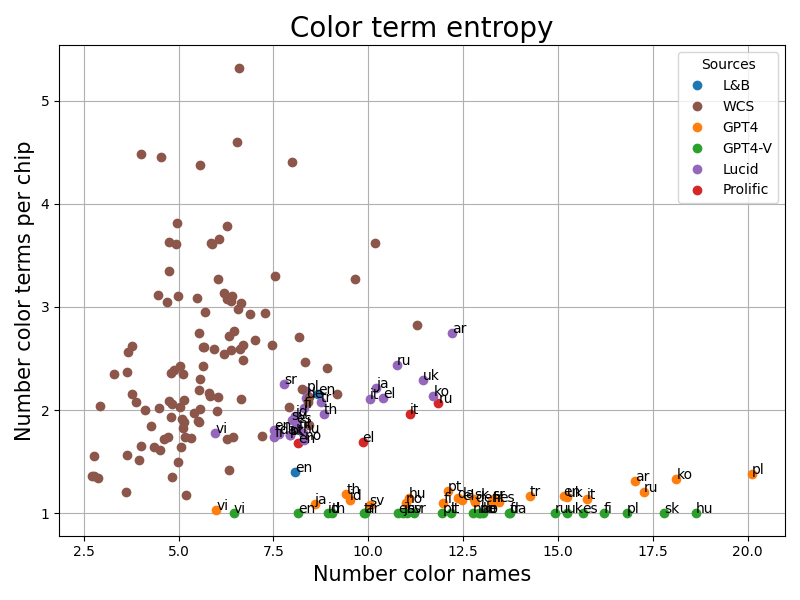
\includegraphics[page=1, width=\linewidth]{images/MDS/entropy-plot.png}
% \decoRule
% \caption[Entropy Plot]{}
% \label{fig:entropy_plot}
% \end{figure}

% \begin{figure}[h!t]
% \centering
% 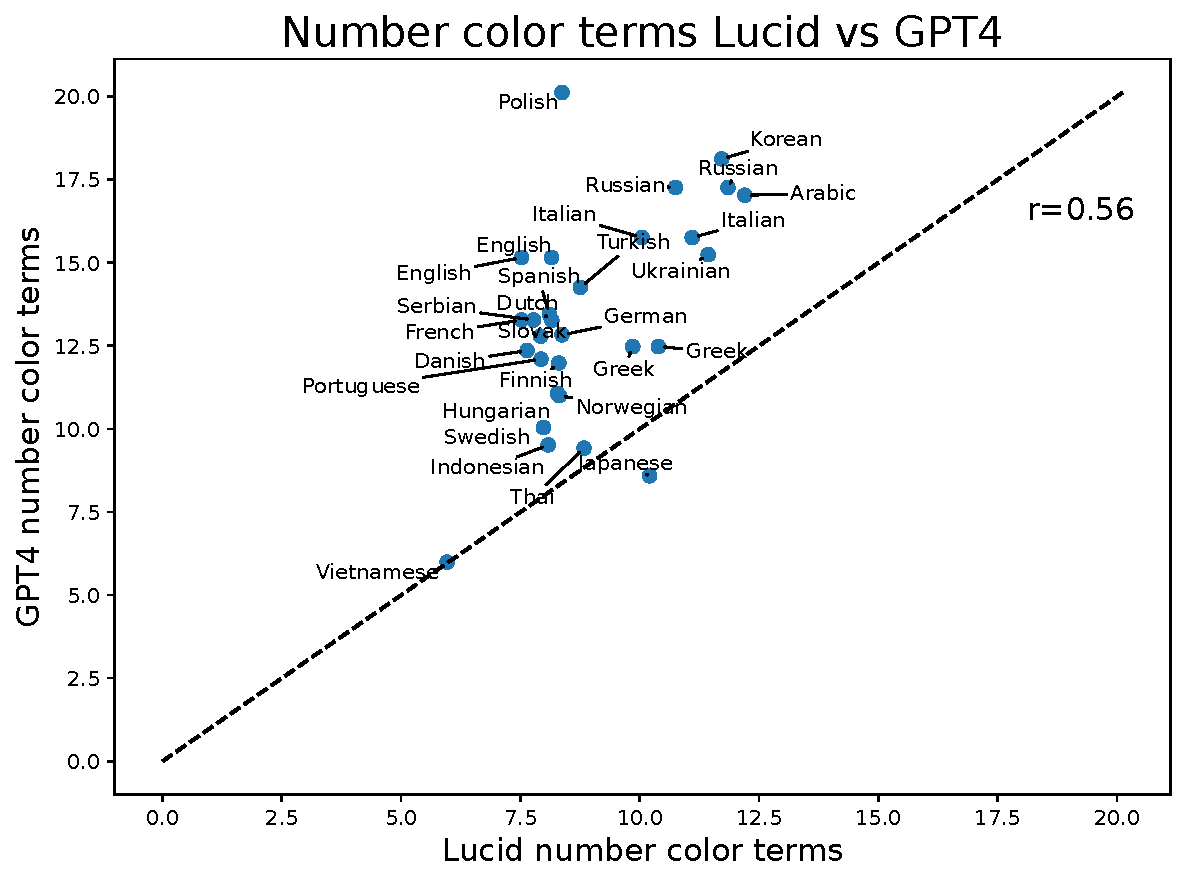
\includegraphics[page=1, width=\linewidth]{images/human_vs_gpt4.pdf}
% \decoRule
% \caption[Number Color Terms: GPT4 vs Human]{}
% \label{fig:human_vs_gpt4}
% \end{figure}

% \begin{figure}[h!t]
% \centering
% 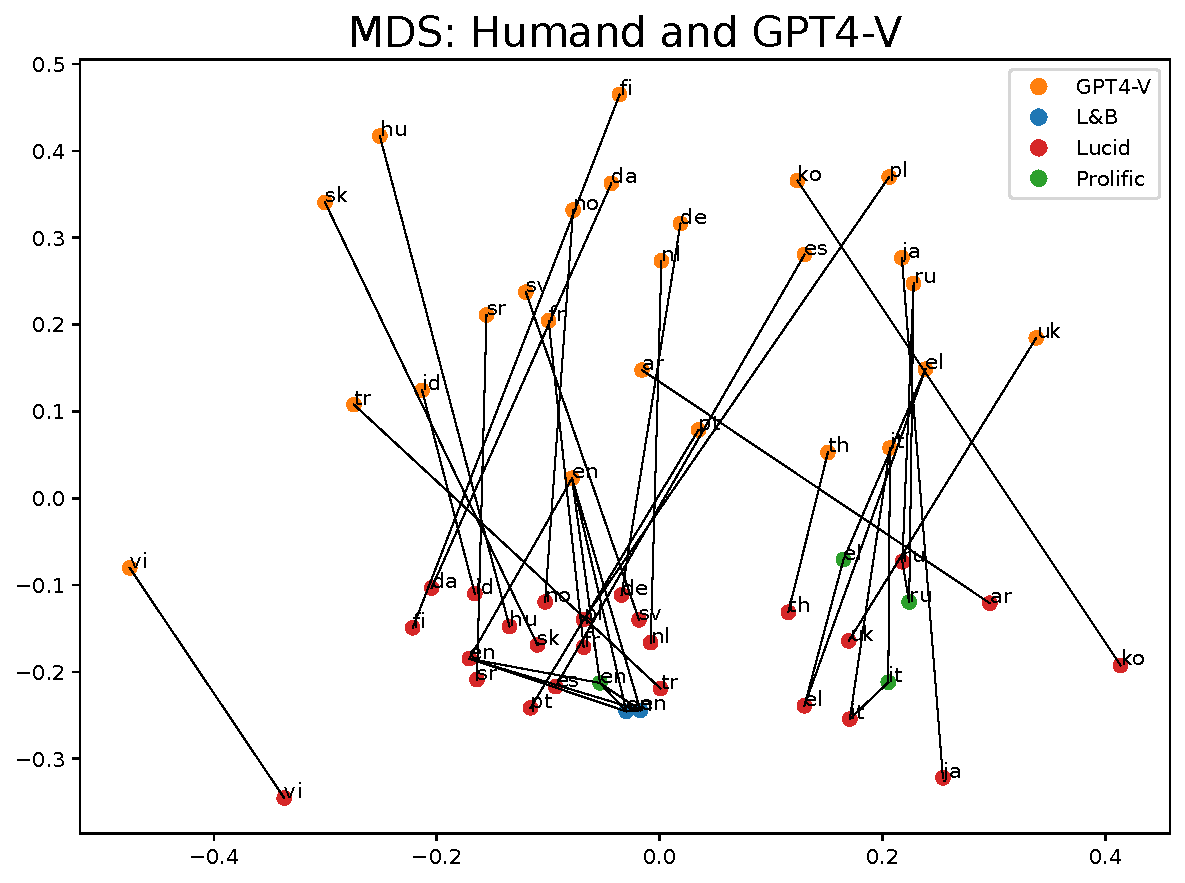
\includegraphics[page=1, width=0.49\linewidth]{images/MDS/mds_rand_index_human_gpt4-v.pdf}
% \hfill
% 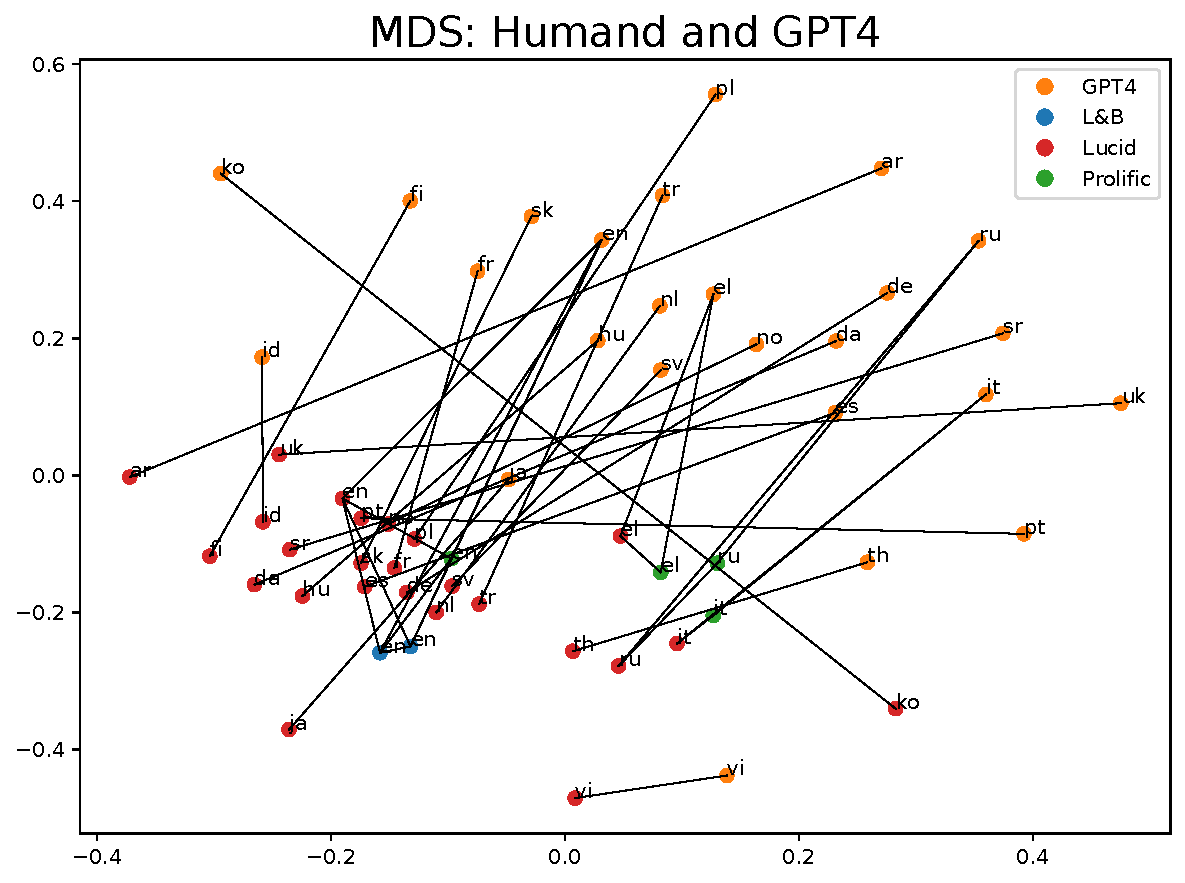
\includegraphics[page=1, width=0.49\linewidth]{images/MDS/mds_rand_index_human_gpt4.pdf}
% \decoRule
% \caption{}
% \label{fig:MDS_human-gpt}
% \end{figure}


% The proportional plots of the GPT4 data exhibit similar but more detailed naming pattern than the human data (Fig. \ref{mode-maps-gpt}.
% For English the BCT are present but subdivided by additional niche categories such as mint, navy, olive, teal and turquoise in the blue and green area. This results in a richer color lexicon of eleven additional terms compared to the human data (global entropy).
% The plots also illustrate low entropy in the responses for each chip (local entropy). Compared to human data, the individual chips show fewer different colors, reflecting a more uniform way of responding.

% Fig. \ref{fig:entropy_plot} illustrates the relationship between the local entropy on the y-axis representing consensus across answers for the single chips and the global entropy on the x-axis defined as the number of color terms in the overall dataset (exponent of the entropy on all chips).
% The different datasets cluster in different areas of the plot highlighting different naming behaviour for GPT4, GPT4-V, WCS and the collected dataset.

% The observations from above get reflected in this plot. GPT4 (orange) data cluster around regions of low local entropy reflecting the highly deterministic naming manner.
% For GPT4-V (green) we only have one answer per color which is why the local entropy equals one for all languages.
% Both human datasets cluster around higher values of local entropy. 
% The languages of the collected data (purple) use significantly more diverse color names per chip compared to GPT4 and GPT4-V (W = .0, p < 0.001 and W = .0, p < 0.001 using Wilcoxon-Rank test).
% In contrast examination of the number of color terms (global entropy, Fig. \ref{human_vs_gpt4}) used by GPT4 and GPT4-V is significantly higher than in the collected human data (W = .0, p < 0.001 and W = .0, p < 0.001 using Wilcoxon-Rank test).
% % Or: (Wilcoxon signed rank test: t(24) = 5.0, p < 0.001, and t(24) = 3.0, p < 0.001)
% However, we see that the number of color categories tend to be correlated across GPT-4-V and humans (r =.09) but not across GPT-4 and humans (r=.55), indicating that languages with a small number of categories in humans (such as Vietnamese) also tend to have fewer categories in GPT-4-V and vice versa.

% When comparing the human data we see a significant higher number of color terms in the newly collected data (9.02 [5.92, 12.12]) than in the WCS data (5.71 [2.57, 8.85]; p < 0.001)







% Also, on a single language level, humans fairly overlap with the labels proposed by GPT-4 (mean: 59\%, SD: 16\%), and the overlapping
% colors occur at a similar frequency except for Arabic (r = .06)
% and Dutch (r = .32) (.44-.90, mean: .65, SD: .13).


